\section{Site graphs}

\subsection{The category of site-graphs}

Define $\kn = \{A, B,..\}$ a set of agent types %with a distinct agent type \emph{free},
and equipped with a site map $\site:\kn\to\nat$.
%such that $\site(\text{free}) = 0$.
Define $\pn$ a set of properties.

%Define the set of external links as follows:
%\[
%\text{Ext} = \set{-,\sfree}\cup\Sigma_{ag}\cup\set{(A,i) : A\in\Sigma_{ag}, i\in\site(A)}
%\]

\begin{definition}[Site-graphs]
\label{def:site_graphs}
A site-graph is a structure $(\ag,\type,\nodes,\links,p_k)$ where
\begin{itemize}
\item $\ag$ is a set of agents, ranged over by $a,b$;
\item $\type:\ag\to \set{A, B,...}$ assigns a type to each agent;
\item $\nodes\subseteq \ag\times\nat\uplus\{\text{free}\}$ is a set of nodes, with a special node free, and where each other node is a pair $(a,i)$ with $a\in\ag$ an agent and $i<\site(\type(a))$ a site of $a$;
\item $\links\subseteq \nodes\times\nodes$ is a set of edges that is \emph{conflict free}: $\forall \xi,\xi'\in\links$, $\xi=\xi'$ or $\xi\cap \xi' \subseteq \{\text{free}\}$;
\item $p_k\subseteq\nodes$, with $k\in\pn$, is the set of internal states of a site. The pairwise intersection of $\{p_k\}_{k\in\pn}$ is the empty set, that is a site can only have one internal state.
\end{itemize}
Denote $\varepsilon$ the empty $\Sigma$-graph.
\end{definition}

\begin{definition}[Morphisms]
\label{def:site_morph}
A morphism $h:G\to H$ is a total function on agents $h:\ag_G\to\ag_H$ such that
\begin{itemize}
\item it preserves agent's types:
\[
\type(a) = \type(h(a)) \text{ for all }a \in \ag_G
\]
\item it preserves nodes:
\[
\text{ if }(a,i)\in \nodes_G \text{ then }(h(a),i) \in \nodes_H\text{ and }h(\text{free})=\text{free}
\]
%% \item it preserves links:
%% \[
%% \text{ if }\epsilon\in \links_G \text{ then }h(\epsilon)\in\links_H
%% \]
\item it preserves property sets:
\[
\set{h(u) : u\in p_{k,G}} \subseteq p_{k,H}, \forall k\in\pn.
\]
\end{itemize}
An embedding or a mono, denoted $h:G\lemb H$, is an injective morphism on edges, that is it preserves edges:
\[
(u,v)\in\links_G \implies (h(u),h(v))\in\links_H
\]
\end{definition}

\begin{lemma}
  Site-graphs and morphisms form a category.
\end{lemma}
\begin{proof}
  The category of site graphs has as objects the site graphs of~\autoref{def:site_graphs} and arrows are the morphisms of~\autoref{def:site_morph}.
%
  Given three site graphs $G_1,G_2,G_3$ and two morphisms $f:G_1\to G_2$, $g:G_2\to G_3$ let $h=f\cdot g$ be the composition of the two. It is defined as follows
  \begin{itemize}
  \item $f\cdot g$ is the composition of $f$ and $g$ on agents;
  \item for $a\in\ag_{G_1}$, $\type(h(a))=g(f(\type(a))$ and we have that $\type(h(a))=h(\type(a))$;
  \item for $(a,i)\in\nodes_{G_2}$, $h(a,i) = g(f(a,i))$ and therefore $h(a,i)=(g(f(a)),i)=(h(a),i)$;
  \item for any $k\in\pn$, $\{h(u): u\in p_{k,G_1}\}=\{f(g(u)): u\in p_{k,G_1}\}$ and we have that $\{g(v): v\in p_{k,G_2}\}\subseteq p_{k,G_3}$ and $\{f(u): u\in p_{k,G_1}\}\subseteq p_{k,G_2}$, hence $\{h(u): u\in p_{k,G_1}\}\subseteq p_{k,G_3}$.
  \end{itemize}
  If $f$ and $g$ are injective, then so is $h$.
%
  The axioms of associativity and identity law easily hold.
\end{proof}

\begin{definition}[Rules]
  \label{def:rule_site}
  A rule is a span $L\overset{h}{\remb} D \overset{g}{\lemb} R$ such that $h$ and $g$ are monos on site graphs and the following hold
  \begin{itemize}
   %\item for any span $L\overset{h'}{\remb} D' \overset{g'}{\lemb} R$ and any embedding $D\overset{f}{\lemb}D'$ such that $h=h'f$ and $g=g'f$ then $f$ is an isomorphism;
  \item $\forall a\in\ag_D$, $(a,i)\in\nodes_D\iff (h(a),i)\in\nodes_L \iff (g(a),i)\in\nodes_R$;
  \item $\forall a\in\ag_D$, $(a,i)\in\nodes_D$ then $[(g(a),i),x] \in\links_R \iff [(h(a),i),y] \in\links_L$;
    %\item if $[(a,i),x] \in\links_R$ and $\nexists b$ such that $h(b)=a$ or $\nexists y$ such that $[(b,i),y]\in\links_D$ then $x\in\sites_R$;
  \item if $a\in\ag_R$ and $a\notin\text{image}(g)$ then $\forall i\in\Sigma_{ag-st}(\type(a))$, $(a,i)\in\nodes_R$ and $\exists e\in \links_R$ such that $(a,i)\in e$;
  \item $\forall a\in\ag_D$, $(a,i)\in\nodes_D$ then $(h(a),i)\in p_{k,L}\iff (g(a),i)\in p_{k',R}$.
  \end{itemize}
\end{definition}

The category of site graphs and morphisms does not have all the pushouts. %but does have all pullbacks.

\begin{example}[Inexistence of pushout in the category of site graphs]
  For the two graphs \verb|A(x!1), B(x!1)| and \verb|A(x)| there is no pushout.
\end{example}

\begin{lemma}
  Let $L\overset{h}{\remb} K \overset{g}{\lemb} R$ be a rule and let $M$ and $m:L\emb M$ be a site graph and matching, respectively. The DPO rewriting can be applied whenever the gluing conditions hold.
\end{lemma}
\begin{proof}
  \[
  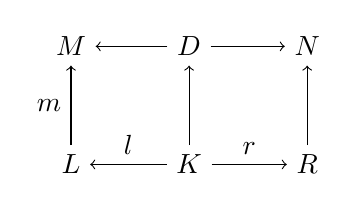
\begin{tikzpicture} %[scale=0.8]
    \node (l) at (-1.5,0) {\(L\)};
    \node (d) at (0,0) {\(K\)};
    \node (r) at (1.5,0) {\(R\)};
    \node (m) at (-1.5,1.5) {\(M\)};
    \node (d') at (0,1.5) {\(D\)};
    \node (n) at (1.5,1.5) {\(N\)};
    \draw [->] (d) -- node [above,midway] {\(l\)} (l);
    \draw [->] (d) -- node [above,midway] {\(r\)} (r);
    \draw [->] (d') -- (m);
    \draw [->] (d') -- (n);
    \draw [->] (l) -- node [left,midway] {\(m\)}  (m);
    \draw [->] (d) -- (d');
    \draw [->] (r) -- (n);
  \end{tikzpicture}
  \]
  Let us first construct $D$ and show that it is a pushout complement. Secondly, we construct $N$ and show that it is the pushout.
  \begin{enumerate}
  \item The graph $D$ is defined as follows:
    \begin{itemize}
    \item $\nodes_D = \nodes_M\setminus m(\nodes_L) \cup m(l(\nodes_K))$
    \item $\links_D = \links_M\setminus m(\links_L) \cup m(l(\links_K))$
    \item $\ag_D = \{a: a\in \text{first}(u), u\in\nodes_D\}$
    \item $p_{k,D} = p_{k,M}\setminus m(p_{k,L}) \cup m(l(p_{k,K}))$
    \end{itemize}
    It is a site graph, because it is a subgraph of $M$, and therefore there is no conflict on the edges and property sets.

    The morphism $f:D\to M$ is defined as the inclusion morphism.
    Let us now show that $D\overset{f}{\leftarrow}M\overset{g}{\rightarrow} L$ is the pushout of the span $L\overset{l}{\rightarrow}K\overset{k}{\leftarrow} D$.
 \begin{mdframed}[backgroundcolor=blue!20]
    to do
  \end{mdframed}

  \item The pushout of the span $R\overset{r}{\rightarrow}K\overset{k}{\leftarrow} D$ is constructed as follow:
    \begin{itemize}
    \item let $\equiv$ be the smallest equivalence relation with $(k(u),r(u))\in\equiv$, for all $u\in\nodes_K$.
    \item $\nodes_N = (\nodes_D\cup \nodes_R)|_{\equiv}$
    \item $\ag_D = \{a: a\in \text{first}(u), u\in\nodes_N\}$
    \item $\links_D = \{(k(u),k(v)) : (u,v)\in\links_K\}\cup\{(r(u),r(v)) : (u,v)\in\links_R\}$
    \item $p_{k,N} = k(p_{k,D}) \cup r(p_{k,R})$
    \end{itemize}
    First let us show that $N$ is a site graph. For that we have to show that $\links_N$ is conflict free. Suppose that there exists $((a,i),(b,j)\in \links_D$ and $((a,i),(c,j)\in \links_R$ and such that $(a,i)\in\nodes_K$. We have then that both $((a,i),(b,j)$ and $((a,i),(c,j)$ are edges in $N$, which are conflicting. However, from the definition of rule (\autoref{def:rule_site}), there exists $x$ such that $((a,i),x)\in\links_K$ and therefore either $k$ or $r$ is not a morphism.
%
    Suppose that there is a conflict in $N$ due to the property sets. For example, let $(a,i)\in p{k,R}$, $(a,i)\in p{k',D}$ and $k\neq k'$. We can reach a contradiction by deriving that $(a,i)\in p{k'',L}$ from \autoref{def:rule_site}.

    Let us now show that $N$ is the pushout.
  \begin{mdframed}[backgroundcolor=blue!20]
    to do
  \end{mdframed}
 \end{enumerate}
 \end{proof}

%\input{influence_kappa.tex}

\begin{lemma}
  Let $\theta$ be a trace and $s=\{E,\tleq,\tprec,\labl\}$ be a story such that $\alpha(\theta) = s$. For any events $e_1,e_2\in E$ if $e_1\prec e_2$ and $e_1\not< e_2$ then there exists $e_3\in E$ such that $e_3\tprec e_2$ and either $e_1< e_3$ or $e_3\dashv e_1$.
\end{lemma}
\begin{proof}
  From~\autoref{def:prec} there exists $t_1:M_1\overset{m_1,p_1}{\Rightarrow} N_1$ and $t_2:M_2\overset{m_2,p_2}{\Rightarrow} N_2$ two transitions such that $\alpha(t_1)=e_1$, $\alpha(t_2)=e_2$ and $\theta:N_1\Rightarrow^{\star}M_2$ a trace between them. Let us first make some remarks.

  First, as $e_1\not< e_2$, the trace $\theta$ is not empty. There exists at least one transition in $\theta$. We consider two cases: there is only one transition in $\theta$ and then the more general case of more than one transition.

  The second remark is that~\autoref{lem:prec} implies that there exists $R_1\leftarrow O\rightarrow L_2$ be a span of injective morphisms such that $O$ is not contained in $D_1$. From $e_1\prec e_2$ and $e_1\not< e_2$ we have that the pushout of the span $R_1\leftarrow O\rightarrow L_2$ is not a site graph. Let us suppose w.l.o.g. that there exists two edges $\xi_1=((a,i), \text{free})$ in $R_1$ and $\xi_2=((a,i),(b,j))$ in $L_2$ that are in conflict. Because of the injective morphisms, we have that $n_1(\xi) \in M_1$ and $m_2(\xi_2)\in M_2$.

  Let us first suppose that there is only one transition and show that the hypothesis hold. We have the following diagram:
  \[
  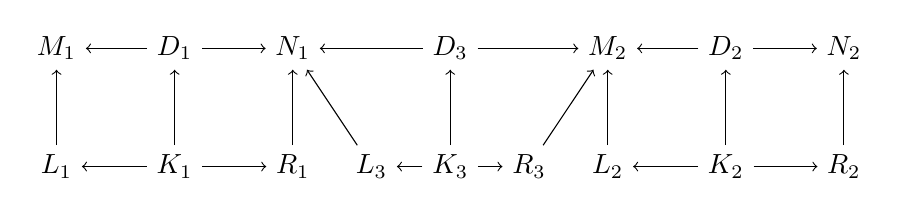
\begin{tikzpicture} %[scale=0.8]
    \node (l1) at (-1.5,0) {\(L_1\)};
    \node (k1) at (0,0) {\(K_1\)};
    \node (r1) at (1.5,0) {\(R_1\)};
    \node (m1) at (-1.5,1.5) {\(M_1\)};
    \node (d1) at (0,1.5) {\(D_1\)};
    \node (n1) at (1.5,1.5) {\(N_1\)};
    \draw [->] (k1) -- (l1);
    \draw [->] (k1) --  (r1);
    \draw [->] (d1) -- (m1);
    \draw [->] (d1) -- (n1);
    \draw [->] (l1) -- (m1);
    \draw [->] (k1) -- (d1);
    \draw [->] (r1) -- (n1);
    \node (l2) at (5.5,0) {\(L_2\)};
    \node (k2) at (7,0) {\(K_2\)};
    \node (r2) at (8.5,0) {\(R_2\)};
    \node (m2) at (5.5,1.5) {\(M_2\)};
    \node (d2) at (7,1.5) {\(D_2\)};
    \node (n2) at (8.5,1.5) {\(N_2\)};
    \draw [->] (k2) -- (l2);
    \draw [->] (k2) --  (r2);
    \draw [->] (d2) -- (m2);
    \draw [->] (d2) -- (n2);
    \draw [->] (l2) -- (m2);
    \draw [->] (k2) -- (d2);
    \draw [->] (r2) -- (n2);
    \node (l3) at (2.5,0) {\(L_3\)};
    \node (k3) at (3.5,0) {\(K_3\)};
    \node (r3) at (4.5,0) {\(R_3\)};
    \node (d3) at (3.5,1.5) {\(D_3\)};
    \draw [->] (k3) -- (l3);
    \draw [->] (k3) --  (r3);
    \draw [->] (d3) -- (n1);
    \draw [->] (d3) -- (m2);
    \draw [->] (l3) -- (n1);
    \draw [->] (k3) -- (d3);
    \draw [->] (r3) -- (m2);
  \end{tikzpicture}
  \]
We have that $n_1(\xi_1)\notin D_3$, as otherwise $n_1(\xi_1)\in M_2$ and it would lead to a conflict.
Then $n_1(\xi_1) \in M_1$, $n_1(\xi_1)\notin D_3$ and $M_1$ the pushout of the span $L_3\leftarrow K_3\rightarrow D_3$. Therefore $m_3^{-1}(n_1(\xi_1)) \in L_3$. Similarly we have that $n_3^{-1}(m_2(\xi_2))\in R_3$ and it follows that $e_3\redl{+}_{O_2} e_2$, with $(\xi_2) \in O_2$.

Remember that $\xi_1\in R_1$ and $m_3^{-1}(n_1(\xi_1)) \in L_3$. We distinguish two cases:
\begin{itemize}
\item if $r_1^{-1}(\xi)\in D_1$ and hence in $L_1$ then we have that $e_3\redl{-}_{O_1} e_1$ with $\xi_1\in O_1$;
\item otherwise we have that $e_1\redl{+}_{O_1} e_3$, again with $\xi_1\in O_1$.
\end{itemize}

Because the influence relations are defined on events in the trace $\theta$, we can use~\autoref{lem:completeness_causal_pair} and~\autoref{lem:completeness_inhib_pair} to obtain that in the trace $\theta$ $e_3< e_2$ and either $e_1 < e_3$ or $e_3\dashv e_1$.

\bigskip

Let us now suppose that there are more than one event in the trace $\theta$. We have seen from the second remark at the beginning at $n_1(\xi_1)\in M_1$ and $m_2(\xi_2)\in M_2$. There exists an event that removes $n_1(\xi_1)$, but from~\autoref{def:rule_site}, second condition, the event either remove the node $(a,i)$ altogether or it keeps an edge $\xi_3$ with $(a,i)\in\xi_3$.
We denote this event $e_3$.

Event $e_3$ cannot remove node $(a,i)$ as $(a,i)\in \nodes_{L_2}$. Therefore $e_3\tprec e_2$. From an argument similar to the first case, we have that either $e_1< e_3$ or $e_3\dashv e_1$.
\end{proof}

\begin{example}
%In site graph we can express a dependence between events that is neither sequential dependence nor inhibition. It comes from the distinction between low res and medium res influence.
Let us consider an example, with the following three rules
\begin{verbatim}
  r1: C(y),A(x!1,y),B(x!1)-> C(y!2),A(x!1,y!2),B(x!1)
  r2: A(x!1), B(x!1) -> A(x), B(x)
  r3: C(y!2),A(x,y!2) -> C(y!2),A(x~p,y!2)
\end{verbatim}

We have that $r_1\xrightarrow[low]{+} r_3$, $r_2\xrightarrow[medium]{+} r_3$ and $r_2\xrightarrow[medium]{-} r_1$.

Let $e_1$, $e_2$ and $e_3$ be three events such that $r_1$, $r_2$ and $r_3$ are their corresponding labels.
In a trace, $e_1$ and $e_3$ cannot occur sequentially, but $e_2$ has to occur in between.
\end{example}

\begin{remark}[Comparison with asymmetric conflict and inhibition in~\cite{BaldanThesis}]
  In both event structures with asymmetric conflict and inhibition, the configurations are downward closed w.r.t. $\leq$, whereas we need sets closed w.r.t. $\tprec$. Another difference is that inhibition in the event structures of~\cite{BaldanThesis} is connected to the causal relation $e_1 < e_2 \implies e_2\dashv e_1$, which is not true in our stories. Lastly, there is no relation in these event structures that can express $\prec$.
\end{remark}

\begin{mdframed}[backgroundcolor=blue!20]
  \begin{itemize}
  \item no context of inihibition: detect conflict in the site graph.
  \end{itemize}
\end{mdframed}
